\documentclass[tikz]{standalone}

\usepackage{pgfplots}
\pgfplotsset{compat=1.15}
\usepackage{mathrsfs}
\usetikzlibrary{arrows,calc}
\usepackage{tkz-euclide}
\pagestyle{empty}

\definecolor{AngleClr}{rgb}{0,0.39215686274509803,0}
\definecolor{ShapeClr}{rgb}{0.6,0.2,0}
\definecolor{BlueSqr}{RGB}{5,81,163}

\begin{document}

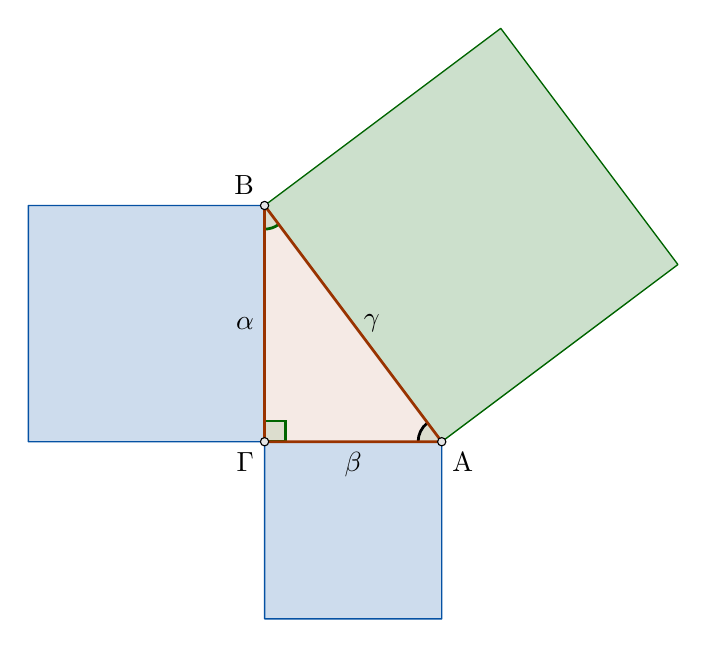
\begin{tikzpicture}[scale=.75]
\tkzSetUpLine[line width=1pt,color=black]

% Ορισμός των συντεταγμένων των κορυφών του τριγώνου.
\tkzDefPoints{0/0/C,0/4/B,3/0/A}

% Χρωματισμός του τριγώνου.
\tkzFillPolygon[fill=ShapeClr,fill opacity=0.1](A,B,C)

\tkzDefSquare(C,B)
\tkzDrawPolygon[fill=BlueSqr,color=BlueSqr,fill opacity=0.2,line width=0.5pt](C,B,tkzFirstPointResult, tkzSecondPointResult)
\tkzDefSquare(A,C)
\tkzDrawPolygon[fill=BlueSqr,color=BlueSqr,fill opacity=0.2,line width=0.5pt](A,C,tkzFirstPointResult, tkzSecondPointResult)

\tkzDefSquare(B,A)
\tkzDrawPolygon[fill=AngleClr,color=AngleClr,fill opacity=0.2,line width=0.5pt](B,A,tkzFirstPointResult, tkzSecondPointResult)

% Επισήμανση γωνιών.
\tkzMarkRightAngle[line width=1pt, size=.35,color=AngleClr,fill=AngleClr,fill opacity=0.1](B,C,A)
\tkzFillAngle[fill=AngleClr,size=.4,fill opacity=0.1](C,B,A)
\tkzMarkAngle[line width=1pt,size=.4,color=AngleClr](C,B,A)
\tkzFillAngle[fill=AngleClr,size=.4,fill opacity=0.1](B,A,C)
\tkzMarkAngle[line width=1pt,fill=AngleClr,size=.4,fill opacity=0.1](B,A,C)

\tkzDrawPolygon[color=ShapeClr](A,B,C)
\tkzDrawPoints[size=3](A,B,C)

% Ονόματα για τις κορυφές του τριγώνου.
\tkzLabelPoint[below right](A){$\rm A$}
\tkzLabelPoint[above left](B){$\rm B$}
\tkzLabelPoint[below left](C){$\rm \Gamma$}

% Ονόματα για τις πλευρές του τριγώνου.
\tkzLabelSegment[right](A,B){$\gamma$}
\tkzLabelSegment(A,C){$\beta$}
\tkzLabelSegment[left](B,C){$\alpha$}

\end{tikzpicture}

\end{document}
